
%----------------------------------------------------------------------------------------
%	PACKAGES AND DOCUMENT CONFIGURATIONS
%----------------------------------------------------------------------------------------

\documentclass{article}

\usepackage{mhchem} % Package for chemical equation typesetting
\usepackage{siunitx} % Provides the \SI{}{} command for typesetting SI units

\usepackage{graphicx} % Required for the inclusion of images

\setlength\parindent{0pt} % Removes all indentation from paragraphs

\renewcommand{\labelenumi}{\alph{enumi}.} % Make numbering in the enumerate environment by letter rather than number (e.g. section 6)

%\usepackage{times} % Uncomment to use the Times New Roman font

%----------------------------------------------------------------------------------------
%	DOCUMENT INFORMATION
%----------------------------------------------------------------------------------------

\title{Creation an account in Emulab } % Title

\author{Rub�n P�rez Pascual} % Author name

\date{\today} % Date for the report

\begin{document}

\maketitle % Insert the title, author and date

\begin{center}
\begin{tabular}{l r}
Date Performed: & February 4, 2014 \\ % Date the experiment was performed
Partners: & Jonathan Becedas \\ Gerardo \"TATA MARTINO\"
& Rub�n P�rez Pascual \\
Instructor: & Jonathan Becedas
\end{tabular}
\end{center}

% If you wish to include an abstract, uncomment the lines below
% \begin{abstract}
This document shows how we can create an account in Emulab\ref{emulab}, to get an X509 certificate and to take to use the Fed4Fire�s testbeds.
% \end{abstract}

%----------------------------------------------------------------------------------------
%	SECTION 1
%----------------------------------------------------------------------------------------

\section{Introducction}

Fed4Fire works with X509 certificates to authenticate experimenters on testbeds. We will register ourselves in Fed4Fire�s page and we will 
create an account.

%----------------------------------------------------------------------------------------
%	SECTION 2
%----------------------------------------------------------------------------------------

\section{Register for an account}

First, we must go at \href{http://www.wall2.ilabt.iminds.be.}. Browser shows this page:

\begin{figure}
\begin{center}
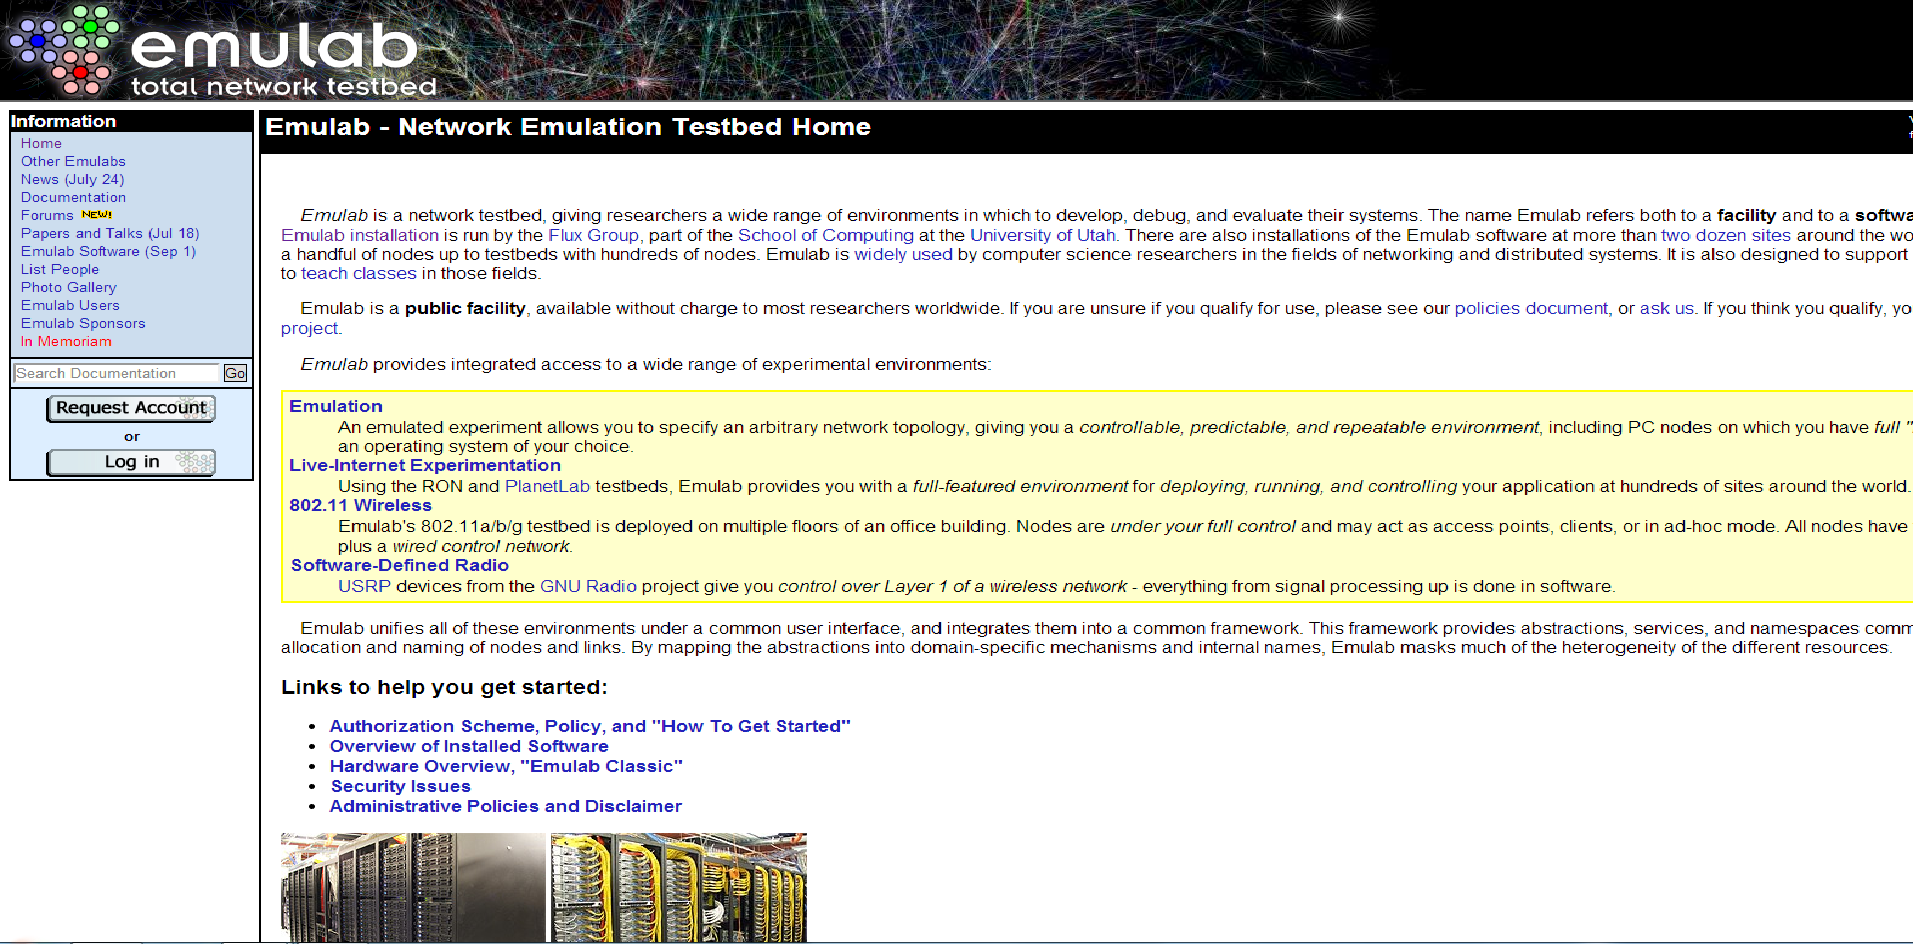
\includegraphics[with = 0.5\textwidth]{figures/homepage.png}
\begin{center}
\end{figure}

At the left side, we click on \emph{Request Account}
We have to create a \emph{Start a New Proyect}. 
Then, we must to fill the form with our account information.

\begin{figure}
\begin{center}
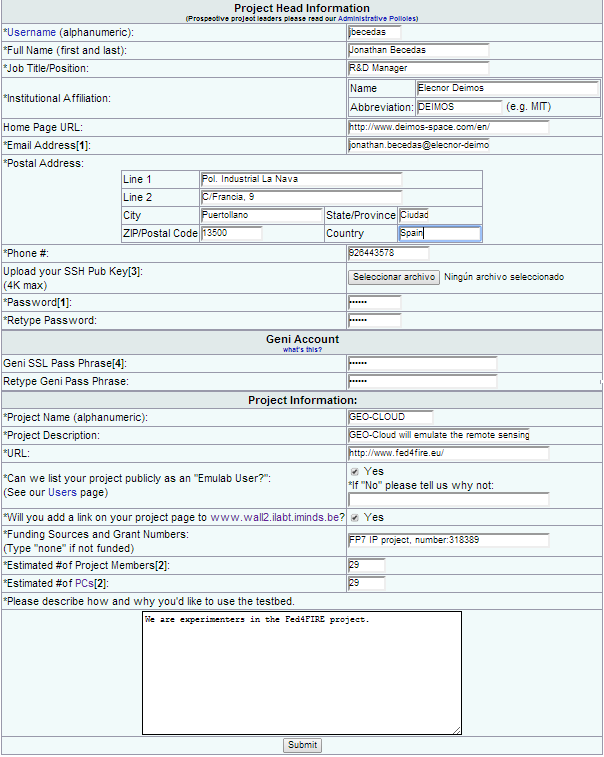
\includegraphics[with = 0.5\textwith]{figures/form.png}
\end{center}
\end{figure}

Username : jbecedas
Password : deimos_space14

%----------------------------------------------------------------------------------------
%	SECTION 3
%----------------------------------------------------------------------------------------

\section{Approve the account}

The next step is managed by the Emulab administrator. In some time, we receive a confirmation email, that it include 
a link for to make our account active.

Once we have the account active, we can to get the SSL certificate by some ways. 
We will download the certificate in PEM format and put in PUTTY and we also get the pkc12 certificate for our browser.

%----------------------------------------------------------------------------------------
%	BIBLIOGRAPHY
%----------------------------------------------------------------------------------------

\bibliographystyle{unsrt}

\bibliography{sample}

%----------------------------------------------------------------------------------------


\end{document}